\documentclass[aspectratio=169,11pt]{beamer}
% Based on the user's attached main(1).tex. Compile twice with pdflatex.
\usetheme{Madrid}
\usecolortheme{whale}
\setbeamertemplate{navigation symbols}{}
\setbeamertemplate{caption}[numbered]
\setbeamerfont{footnote}{size=\tiny}

\usepackage[T1]{fontenc}
\usepackage[utf8]{inputenc}
\usepackage{lmodern,amsmath,amssymb,graphicx,booktabs,array,listings,pgfplots}
\usepgfplotslibrary{groupplots}
\pgfplotsset{compat=1.18}
\definecolor{navy}{HTML}{204C70}
\definecolor{burnt}{HTML}{B85932}
\definecolor{teal}{HTML}{28786B}
\definecolor{lightteal}{HTML}{A3C6BC}
\graphicspath{{figures/}}
\setbeamerfont{footnote}{size=\tiny}
\setbeamertemplate{footline}{\leavevmode\hbox{\begin{beamercolorbox}[wd=.73\paperwidth,ht=2.6ex,dp=1ex,leftskip=1em]{author in head/foot}Group 2 \quad CSE-625 \quad Custom Memory Allocator Profiling\end{beamercolorbox}\begin{beamercolorbox}[wd=.27\paperwidth,ht=2.6ex,dp=1ex,rightskip=1em plus1fil]{date in head/foot}\hfill\insertframenumber/\inserttotalframenumber\end{beamercolorbox}}}
\newcommand{\source}[1]{\par\vfill{\tiny\color{gray}#1\par}}
\newcommand{\plotheight}{4.3cm}
\newcommand{\barwidth}{14pt}
\newcommand{\pointsize}{1.3pt}
\newcommand{\takeaway}[1]{\par\medskip{\color{navy}\bfseries #1}\par}
\lstset{basicstyle=\ttfamily\scriptsize,keywordstyle=\color{navy},commentstyle=\itshape\color{gray},breaklines=true,showstringspaces=false,language=C++}
\title[Allocator Profiling]{Assignment 1 --- Custom Memory Allocator Profiling}
\subtitle{Workload choices, code behavior, and statistical evidence}
\author[Group 2]{Jacob Nance \quad Fernanda Gonzalez \quad Francisco Chagua\\[.3em]Nicholas Hooper \quad Nicholas Johnson \quad Mohamed Konsowa}
\usepackage{lmodern}
\usepackage{amsmath}
\usepackage{amssymb}
\usepackage{graphicx}
\graphicspath{{figures/}{../figures/}}
\usepackage{booktabs}
\usepackage{tikz}
\usepackage{pgfplots}
\pgfplotsset{compat=1.18}

\title[Group 2 --- CMA]{Custom Memory Allocator Profiling}
\subtitle{CSE-625 Assignment 1 --- Group 2}
\author[Group 2]{%
    Jacob Nance \quad Fernanda Gonzalez \quad Francisco Chagua \\[0.3em]
    Nicholas Hooper \quad Nicholas Johnson \quad Mohamed Konsowa
}
\institute[CSE-625]{CSE-625 --- Fall 2026}
\date{September 22, 2026}

\begin{document}
\begin{frame}[plain]\titlepage\end{frame}
\begin{frame}{Research questions}
\begin{enumerate}
\item How did each version track free memory, handle memory blocks, align allocations, and account for metadata?
\item What advantages and costs did those choices carry for fragmentation, allocation search cost, and lock contention?
\item What costs did specializing a version for matrix arithmetic create for other allocation patterns?
\item Could a simpler multi-threaded implementation be made competitive by pairing it with the custom allocator?
\end{enumerate}
% \takeaway{The evidence supports workload-specific gains, with important failures and limits.}
\source{Report Sections I, III, XII and XIV. Updated v8 analyses, September 22.}
\end{frame}


\begin{frame}{Why exhaustive profiling is impractical}
A full search would cross allocator versions, request sizes, object lifetimes, thread counts, hardware, OS, compiler, and machine state.
\medskip
\begin{itemize}
\item Even a simplified plan requires $8\times4\times3\times2\times5=960$ runs per environment: versions, workloads, scales, allocators, repeats.
\item This is an illustrative complete design, not the number of completed measurements.
\item Long runs take hours. More combinations also change thermal state, memory pressure, and background activity.
\end{itemize}
\takeaway{We sampled distinct allocation behaviors and compared matched programs within each environment.}
\source{Report Sections IV, VI and XIV. The 960-run calculation illustrates the design space.}
\end{frame}


\begin{frame}{Four workloads cover different allocation behaviors}
\small\centering
\begin{tabular}{p{.20\textwidth}p{.34\textwidth}p{.35\textwidth}}\toprule
Workload & Allocation pattern & Mechanism tested\\\midrule
Matrix array & Repeated matrix rows & Row placement and arithmetic cost\\
Uniform nodes & Repeated sizes plus node churn & Reuse and cache refill\\
Nested matrix stress & Mixed sizes and branch rebuilds & Fragmentation and coalescing\\
Linked list & Tiny objects, frequent updates & Metadata and search overhead\\
\bottomrule\end{tabular}\par
\medskip\raggedright
\normalsize The suite tests representative mechanisms. It does not establish that any version is best for all applications.
\source{Report Section VI, workload headers described in the report.}
\end{frame}


\begin{frame}{Comparison protocol and run-length labels}
\begin{itemize}
\item Regular and Overloaded use the same workload source, arguments, and deterministic input within a comparison.
\item GNU time records elapsed time, peak memory, page faults, CPU use, and context switches. Checksums check output consistency.
\item Many campaigns use five repeats. The existing v8 group has three pairs per size; the new v8 group has five.
\end{itemize}
\medskip
\small\centering
\begin{tabular}{p{.23\textwidth}p{.30\textwidth}p{.36\textwidth}}\toprule
Strategy & What changes & Interpretation\\\midrule
Repeat fixed workload & Number of launches & More duration, similar working set\\
Grow the problem & Matrix or list size & Different memory and arithmetic demands\\
\bottomrule\end{tabular}\par
\takeaway{Short, medium, and long are within-campaign labels, not matched workloads across hosts.}
\source{Report Sections IV and VI-F. New v8 CSV: Arg1 = 275/400/550.}
\note{The newer v8 runs do not meet the original medium/long duration targets. Their labels denote increasing argument size. Pairing follows successive Regular/Overloaded records in each CSV cycle and is assumed.}
\end{frame}


\begin{frame}{Hardware and operating-system coverage}
\small\centering
\begin{tabular}{p{.31\textwidth}p{.32\textwidth}p{.27\textwidth}}\toprule
Campaign / host & Architecture and OS & Scope\\\midrule
Apple M3 Max, 48 GB & ARM64, macOS & Matrix v1--v7, v6 suite, v8 E1\\
Ryzen 9 7900X, 32 GB & x86-64, Ubuntu under WSL & v7 four-workload suite\\
Intel i7-1165G7, 16 GB & x86-64, Ubuntu 24.04.3 & Jacob v2 and new v8 E2\\
Intel i7-11370H, 16 GB & x86-64, WSL and Linux Mint & 8-thread pthread comparison\\
Shared-team inventory & M5 Pro, other Intel and Ryzen & macOS, Arch Linux, WSL\\
\bottomrule\end{tabular}\par
\medskip\raggedright\normalsize
Two arches (\textbf{ARM64}, \textbf{x86-64}) and several OS runtimes
(\textbf{macOS}, \textbf{WSL}, \textbf{native Linux}), plus shared-team hosts.
\takeaway{Versions and parameters are not balanced across hosts --- compare within an environment.}
\source{Report Tables II--V and XXII--XXIII, Section XII. Updated v8 inventory.}
\note{Some inventory fields are missing. Campaign IDs on the M3 Max denote runs on the same Mac, not separate machines. OS and toolchain versions also differ by campaign.}
\end{frame}


\begin{frame}{Statistical evidence beyond descriptive summaries}
\small\centering
\begin{tabular}{p{.27\textwidth}p{.35\textwidth}p{.29\textwidth}}\toprule
Question & Method & What it establishes\\\midrule
Regular vs Overloaded & Paired, two-condition ANOVA & \textbf{How big} the mean within-pair gap is\\
More increases than decreases? & Directional $\chi^2$; exact sign test & \textbf{How often} one side wins (direction only)\\
v8 groups across environments & Welch ANOVA on paired \% changes & Whether \% changes differ by group\\
Four pthread methods & One-way ANOVA + Tukey HSD & Which methods differ (pairwise-adjusted)\\
Assumptions and scaling & Shapiro--Wilk, Levene, fitted models & Diagnostics and descriptive growth\\
\bottomrule\end{tabular}\par
\medskip\raggedright\normalsize
Means still report typical time; these tests ask whether the pattern is reliable.
Significance uses $\alpha=0.05$. A small $p$ is not effect size and not a causal proof.
\source{Report VII and XII. Updated v8 methods. Tukey controls its pairwise family; v8 p values are unadjusted.}
\end{frame}


\begin{frame}{Allocator evolution: search and reuse}
\small\centering
\begin{tabular}{p{.09\textwidth}p{.54\textwidth}p{.28\textwidth}}\toprule
Version & What changes (CMA intercepts \texttt{new}/\texttt{delete}) & Tradeoff\\\midrule
v1 & Address-ordered list, \textbf{first-fit}, merge on free & Simple path; list search\\
v2 & Same list, \textbf{best-fit} & Tighter fit; full-list scan\\
v3 & Size bins, bitmap, physical-neighbor metadata & Narrower search; bin bookkeeping\\
v4 & Thread caches, 64 blocks/class, 8192-byte limit & Cheap cache hits; retained memory\\
\bottomrule\end{tabular}\par
\medskip\raggedright\normalsize
These are CMA versions, not ``regular \texttt{new} plus a tweak.''
The public API stays the same; the free-block policy changes.
\source{Report Section III and Table I. Code details are reported descriptions, not a new source-code audit.}
\end{frame}


\begin{frame}{Allocator evolution: deferred work and specialization}
\small\centering
\begin{tabular}{p{.09\textwidth}p{.54\textwidth}p{.28\textwidth}}\toprule
Version & What changes & Tradeoff\\\midrule
v5 & Merge only after allocation cannot be satisfied & Cheaper free; expensive miss path\\
v6 & Batch refill up to 32 slabs; \textbf{4 MiB} cache cap & Amortized refill; reserved capacity\\
v7 & Per-class targets grow from 16 to 256 & Adapts to misses; extra accounting\\
v8 & \textbf{Written v8:} keep thread cache; raise cap $256\rightarrow512$;
      retune every 256 allocs; live-block accounting; bin bitmaps
      & Better tiny-object cache; not a packing win\\
\bottomrule\end{tabular}\par
\takeaway{A newer policy can help one pattern and hurt another. AI-generated v8 is separate --- compared later.}
\source{Report Section III and Table I. Written v8 = cache-tuned line from v7.}
\end{frame}


\begin{frame}{What happens when the program requests memory}
\begin{enumerate}
\item Matrix needs a result row $\rightarrow$ each row calls \texttt{new}.
\item Global \texttt{new} routes into the initialized \textbf{custom pool}.
\item Version path checks reuse structures, finds a block, splits when possible.
\item Metadata, alignment, back-pointer, and canaries surround the payload.
\item On \texttt{delete}: ownership + canary checks, then cache or free bins.
      Merge timing depends on the version (v1--v8).
\end{enumerate}
\takeaway{We can describe the path. Total runtime is overall cost --- it does not say how long each step took.}
\source{Report Sections III and VI.}
\note{The singleton uses static storage and placement new to avoid allocator recursion. An uninitialized pool falls back to malloc/posix_memalign. The presentation does not claim to have independently audited the repository.}
\end{frame}


\begin{frame}{Simpler versions led the M3 Max matrix campaign}
\begin{columns}[T]\begin{column}{.69\textwidth}\centering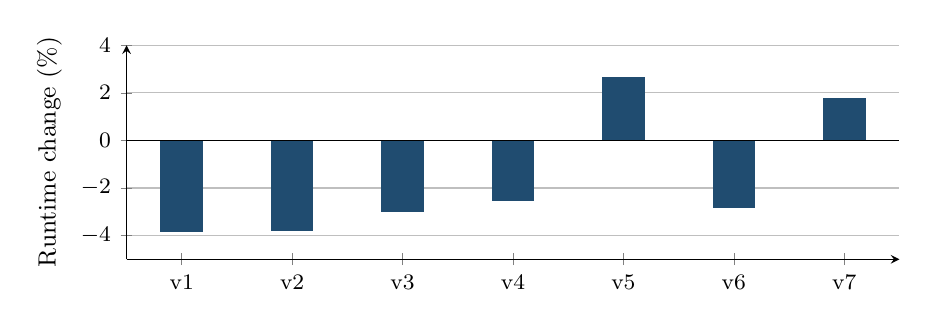
\begin{tikzpicture}\begin{axis}[width=.94\linewidth,height=\plotheight,axis lines=left,tick label style={font=\footnotesize},label style={font=\small},legend style={font=\footnotesize,draw=none},xmin=.5,xmax=7.5,ymin=-5,ymax=4,xtick={1,2,3,4,5,6,7},xticklabels={v1,v2,v3,v4,v5,v6,v7},ylabel={Runtime change (\%)},ymajorgrids=true]
\addplot[ybar,bar width=15pt,fill=navy,draw=navy] coordinates {(1,-3.827693) (2,-3.792639) (3,-2.970204) (4,-2.509101) (5,2.656060) (6,-2.815154) (7,1.758123)};\addplot[black,no marks] coordinates {(.5,0) (7.5,0)};
\end{axis}\end{tikzpicture}\end{column}
\begin{column}{.29\textwidth}\small
Size 360, short runs, three observations per allocator.
\medskip
v1: $-3.83\%$\\v2: $-3.79\%$\\v7: $+1.76\%$
\medskip
Negative change means lower runtime.
\medskip
These descriptive results belong to this campaign, not the shared-workbook v7 environment.
\end{column}\end{columns}
\source{Report Table VI. Six concurrent processes per batch reported in VII-A.}
\end{frame}

\begin{frame}{Environment Significance}
\begin{columns}[T]\begin{column}{\textwidth}\begin{table}[H]\caption{Environment ANOVA}
\centering\tiny\setlength{\tabcolsep}{0.5pt}\renewcommand{\arraystretch}{0.88}
\resizebox{0.90\linewidth}{!}{%
\begin{tabular}{@{}llllcrrr@{}}
\toprule
Version & Workload & Comparison & Env.\ IDs & $n$ & $F$ & $p$ & Sig. \\ \midrule
v7.0.0 & Matrix & All Sizes & 1, 2 & 20 & 60.3979 & $3.6929\times10^{-7}$ & Yes \\
v6.0.0 & Matrix & All Sizes & 1, 2 & 20 & 374.4904 & $1.6999\times10^{-13}$ & Yes \\
v5.0.0 & Matrix & All Sizes & 1, 2 & 25 & 0.6923 & 0.4139 & No \\
v5.0.0 & Uniform Nodes & All Sizes & 1, 2, 3 & 35 & 2,866.2357 & $8.1329\times10^{-37}$ & Yes \\
v4.0.0 & Matrix & All Sizes & 1, 2 & 25 & 0.0879 & 0.7696 & No \\
v4.0.0 & Matrix & Short & 1, 2 & 10 & 35.7068 & $3.3235\times10^{-4}$ & Yes \\
v4.0.0 & Matrix & Medium & 1, 2 & 10 & 1.996 & 0.1954 & No \\
v4.0.0 & Uniform Nodes & All Sizes & 1, 2, 3 & 35 & 3,193.9375 & $1.4520\times10^{-37}$ & Yes \\
v3.0.0 & Matrix & All Sizes & 1, 2 & 15 & 1.452 & 0.2497 & No \\
v2.0.0 & Matrix & All Sizes & 1, 2 & 20 & 4.6506 & 0.0448 & Yes \\
\bottomrule\end{tabular}%
}
\label{EnvAnova}
\end{table}\end{column}\end{columns}
\end{frame}


\begin{frame}{Pthreads experiment: implementation and allocator are separate}
\begin{itemize}
\item Same Intel i7-11370H machine, 16 GB RAM, eight threads, matrix size $n=800$, multiplication involving 200 matrices.
\item \textbf{Pthreads v4}: queues and mutexes, simpler implementation.
\item \textbf{Pthreads v6}: removes those mechanisms to improve locality and throughput, with more implementation complexity.
\item Each runs with Regular new or \textbf{CMA v7}, under Windows WSL and native Linux Mint.
\end{itemize}
\takeaway{Pthreads v4/v6 name workload implementations. CMA v7 names the allocator.}
\source{Report Section XII-A.}
\end{frame}


\begin{frame}{Pthreads runtime depends on the environment}
\centering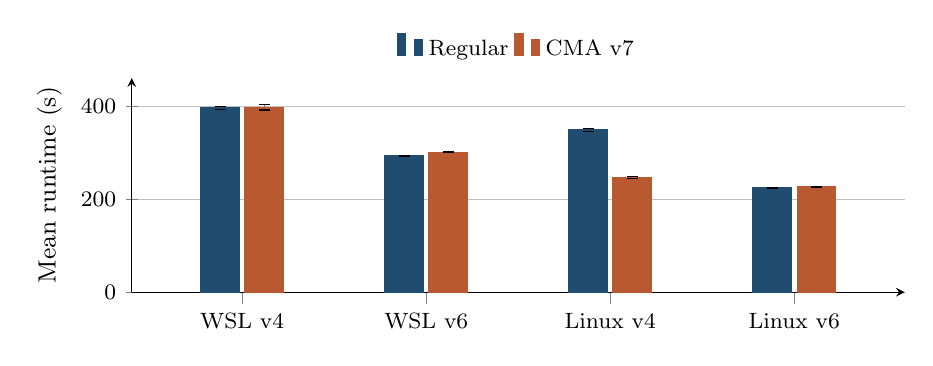
\begin{tikzpicture}\begin{axis}[width=.94\linewidth,height=\plotheight,axis lines=left,tick label style={font=\footnotesize},label style={font=\small},legend style={font=\footnotesize,draw=none},ybar,xmin=-.6,xmax=3.6,ymin=0,ymax=460,xtick={0,1,2,3},xticklabels={WSL v4,WSL v6,Linux v4,Linux v6},ylabel={Mean runtime (s)},legend style={at={(.5,1.03)},anchor=south,legend columns=2},ymajorgrids=true]
\addplot[ybar,bar width=\barwidth,fill=navy,draw=navy,error bars/.cd,y dir=both,y explicit] coordinates {(0,395.795) +- (0,3.762) (1,292.769) +- (0,1.618) (2,348.573) +- (0,2.909) (3,224.896) +- (0,1.057)};\addlegendentry{Regular}
\addplot[ybar,bar width=\barwidth,fill=burnt,draw=burnt,error bars/.cd,y dir=both,y explicit] coordinates {(0,397.664) +- (0,6.023) (1,300.914) +- (0,.627) (2,246.981) +- (0,2.615) (3,226.776) +- (0,.843)};\addlegendentry{CMA v7}
\end{axis}\end{tikzpicture}
\par\small Bars are means and whiskers are sample standard deviations. CMA helps the simpler v4 implementation on native Linux.
\source{Report Tables XII and XVI. Means and SD copied from the report, not recalculated from raw pthread runs.}
\end{frame}


\begin{frame}{Pthreads pairwise tests qualify the claim of worsening}
\small\centering
\begin{tabular}{llrll}\toprule
Environment & Pthreads & CMA change & Tukey $p$ & Significant\\\midrule
WSL & v4 & +0.47\% & 0.8495 & No\\
WSL & v6 & +2.78\% & 0.0135 & Yes\\
Linux & v4 & -29.15\% & $<0.0001$ & Yes\\
Linux & v6 & +0.84\% & 0.4965 & No\\
\bottomrule\end{tabular}\par
\medskip\raggedright\normalsize
\begin{itemize}
\item Under WSL, v6 slows by 2.78\% with CMA. The v4 difference is not significant.
\item Under Linux, CMA reduces v4 runtime by 29.15\%. The v6 difference is not significant.
\end{itemize}
\takeaway{The report does not support a general claim that CMA made pthreads much worse.}
\source{Report Tables XIV and XVIII. Percentage changes calculated from Tables XII and XVI.}
\end{frame}


\begin{frame}{Why allocation policy can hurt parallel matrix work}
\begin{columns}[T]
\begin{column}{.48\textwidth}\textbf{Mechanisms described by the code}
\begin{itemize}\item Cache misses and refills reach a central mutex.\item Search, splitting, and coalescing add work.\item Row layout and metadata change memory access.\item Queue synchronization in pthreads v4 adds another cost.\end{itemize}\end{column}
\begin{column}{.48\textwidth}\textbf{What the measurements establish}
\begin{itemize}\item Runtime differs across method and environment.\item Page-fault and context-switch totals are symptoms, not attribution.\item No lock-wait, cache-miss, or allocation-latency breakdown isolates a cause.\end{itemize}\end{column}\end{columns}
\takeaway{Contention and locality are plausible explanations. They are not directly measured causal findings.}
\source{Report Sections III, XII and XIV.}
\note{Useful next measurements: per-thread allocator call counts, mutex wait time, cache/TLB misses, CPU migrations and time in findBestFit/coalescing. Hardware counters and traces should be collected on matched workloads.}
\end{frame}


\begin{frame}{The report’s scaling graph shows a remaining tradeoff}
\begin{columns}[c]\begin{column}{.52\textwidth}\centering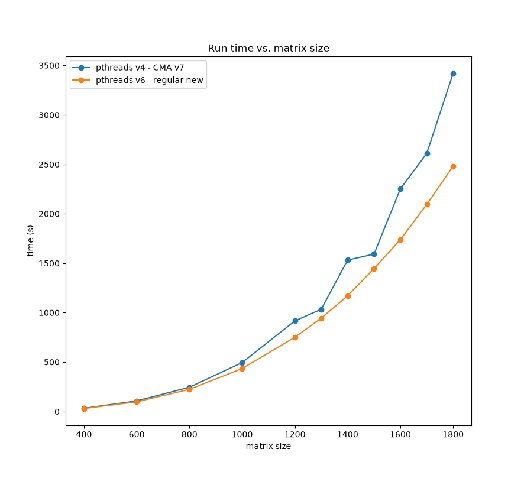
\includegraphics[height=5.6cm]{report_pthreads_scaling.pdf}\end{column}
\begin{column}{.45\textwidth}\small
Native Linux, $n=400$--$1800$.
\medskip
Simpler pthreads v4 + CMA v7 remains about \textbf{8.5--37.9\% slower} than pthreads v6 + Regular over the measured range.
\medskip
Reported power exponents: 3.064 and 2.938.
\medskip
One run per size supports descriptive scaling, not a reliable significance claim at each size. Extrapolation is uncertain.
\end{column}\end{columns}
\source{Original report Figure 5 and Table XXI, p. 19. Figure preserved from the supplied PDF.}
\end{frame}


\begin{frame}{Written v8 vs AI-generated v8}
\small
Group~2 has \textbf{two} v8 designs. Opposite bets.
\medskip
\centering
\renewcommand{\arraystretch}{1.35}
\begin{tabular}{@{}l
  >{\raggedright\arraybackslash}p{0.38\linewidth}
  >{\raggedright\arraybackslash}p{0.38\linewidth}@{}}
\toprule
& \centering\textbf{Written v8} &
  \centering\textbf{AI-generated v8}\tabularnewline
\midrule
Hot path &
  Keeps thread cache; retunes every 256 allocs &
  Skips cache; central best-fit \\
Cache &
  Cap $256\rightarrow512$ / class &
  Off on hot path \\
Arena &
  One mmap (like v7) &
  Small + guard + large \\
Align &
  Page @ 64\,KiB (like v7) &
  64-byte if $\ge$2\,KiB; page only @ 2\,MiB \\
Remainders &
  Round to 64-byte quantum &
  Exact size (packed stride) \\
Focus &
  Better tiny-object cache &
  Pack reused medium matrix rows \\
\bottomrule
\end{tabular}
\par
\medskip\raggedright\normalsize
Matrix result tables later are for the \textbf{AI-generated v8} unless labeled otherwise.
\source{Written v8: cache-tuned from v7. AI-generated v8: packed-row policies profiled on M3 Max / E2.}
\end{frame}


\begin{frame}{V8 Regular versus Overloaded observations}
\centering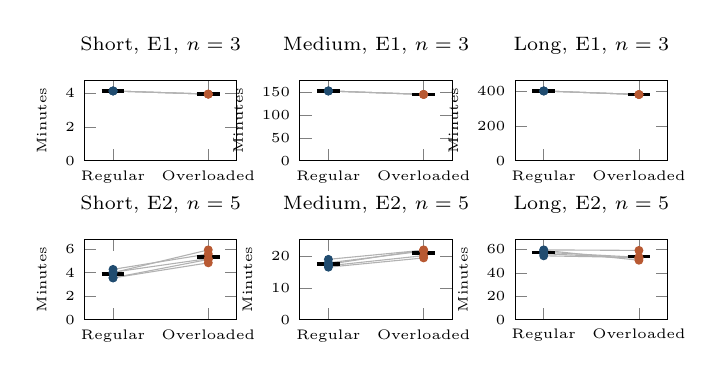
\begin{tikzpicture}\begin{groupplot}[group style={group size=3 by 2,horizontal sep=.8cm,vertical sep=1cm},width=.29\linewidth,height=2.6cm,xmin=-.3,xmax=1.3,ymin=0,xtick={0,1},xticklabels={Regular,Overloaded},tick label style={font=\tiny},title style={font=\scriptsize},ylabel={Minutes},label style={font=\tiny}]
\nextgroupplot[title={Short, E1, $n=3$},ymax=4.755441666666666]
\addplot[gray!60,no marks] coordinates {(0,4.134833333333334) (1,3.9475)};
\addplot[gray!60,no marks] coordinates {(0,4.1339999999999995) (1,3.9478333333333335)};
\addplot[gray!60,no marks] coordinates {(0,4.135166666666667) (1,3.9481666666666664)};
\addplot[only marks,mark=*,mark size=1.4pt,color=navy] coordinates {(0,4.134833333333334) (0,4.1339999999999995) (0,4.135166666666667)};
\addplot[black,very thick,no marks] coordinates {(-0.12,4.134666666666667) (0.12,4.134666666666667)};
\addplot[only marks,mark=*,mark size=1.4pt,color=burnt] coordinates {(1,3.9475) (1,3.9478333333333335) (1,3.9481666666666664)};
\addplot[black,very thick,no marks] coordinates {(0.88,3.947833333333333) (1.12,3.947833333333333)};
\nextgroupplot[title={Medium, E1, $n=3$},ymax=175.52488333333332]
\addplot[gray!60,no marks] coordinates {(0,152.60416666666666) (1,145.02466666666666)};
\addplot[gray!60,no marks] coordinates {(0,152.593) (1,145.02233333333334)};
\addplot[gray!60,no marks] coordinates {(0,152.63033333333334) (1,145.01383333333334)};
\addplot[only marks,mark=*,mark size=1.4pt,color=navy] coordinates {(0,152.60416666666666) (0,152.593) (0,152.63033333333334)};
\addplot[black,very thick,no marks] coordinates {(-0.12,152.60916666666665) (0.12,152.60916666666665)};
\addplot[only marks,mark=*,mark size=1.4pt,color=burnt] coordinates {(1,145.02466666666666) (1,145.02233333333334) (1,145.01383333333334)};
\addplot[black,very thick,no marks] coordinates {(0.88,145.02027777777778) (1.12,145.02027777777778)};
\nextgroupplot[title={Long, E1, $n=3$},ymax=460.11404166666665]
\addplot[gray!60,no marks] coordinates {(0,400.0991666666667) (1,379.66299999999995)};
\addplot[gray!60,no marks] coordinates {(0,400.0315) (1,379.5996666666667)};
\addplot[gray!60,no marks] coordinates {(0,400.055) (1,379.61716666666666)};
\addplot[only marks,mark=*,mark size=1.4pt,color=navy] coordinates {(0,400.0991666666667) (0,400.0315) (0,400.055)};
\addplot[black,very thick,no marks] coordinates {(-0.12,400.0618888888889) (0.12,400.0618888888889)};
\addplot[only marks,mark=*,mark size=1.4pt,color=burnt] coordinates {(1,379.66299999999995) (1,379.5996666666667) (1,379.61716666666666)};
\addplot[black,very thick,no marks] coordinates {(0.88,379.6266111111111) (1.12,379.6266111111111)};
\nextgroupplot[title={Short, E2, $n=5$},ymax=6.840774999999999]
\addplot[gray!60,no marks] coordinates {(0,3.558666666666667) (1,4.843666666666667)};
\addplot[gray!60,no marks] coordinates {(0,3.5631666666666666) (1,5.133666666666667)};
\addplot[gray!60,no marks] coordinates {(0,4.285333333333333) (1,5.600666666666667)};
\addplot[gray!60,no marks] coordinates {(0,4.001) (1,5.948499999999999)};
\addplot[gray!60,no marks] coordinates {(0,4.045) (1,5.2091666666666665)};
\addplot[only marks,mark=*,mark size=1.4pt,color=navy] coordinates {(0,3.558666666666667) (0,3.5631666666666666) (0,4.285333333333333) (0,4.001) (0,4.045)};
\addplot[black,very thick,no marks] coordinates {(-0.12,3.8906333333333336) (0.12,3.8906333333333336)};
\addplot[only marks,mark=*,mark size=1.4pt,color=burnt] coordinates {(1,4.843666666666667) (1,5.133666666666667) (1,5.600666666666667) (1,5.948499999999999) (1,5.2091666666666665)};
\addplot[black,very thick,no marks] coordinates {(0.88,5.347133333333334) (1.12,5.347133333333334)};
\nextgroupplot[title={Medium, E2, $n=5$},ymax=25.305749999999996]
\addplot[gray!60,no marks] coordinates {(0,16.54883333333333) (1,19.467499999999998)};
\addplot[gray!60,no marks] coordinates {(0,16.979499999999998) (1,20.186333333333334)};
\addplot[gray!60,no marks] coordinates {(0,17.910500000000003) (1,21.634999999999998)};
\addplot[gray!60,no marks] coordinates {(0,19.017999999999997) (1,21.90983333333333)};
\addplot[gray!60,no marks] coordinates {(0,17.458333333333332) (1,22.005)};
\addplot[only marks,mark=*,mark size=1.4pt,color=navy] coordinates {(0,16.54883333333333) (0,16.979499999999998) (0,17.910500000000003) (0,19.017999999999997) (0,17.458333333333332)};
\addplot[black,very thick,no marks] coordinates {(-0.12,17.583033333333333) (0.12,17.583033333333333)};
\addplot[only marks,mark=*,mark size=1.4pt,color=burnt] coordinates {(1,19.467499999999998) (1,20.186333333333334) (1,21.634999999999998) (1,21.90983333333333) (1,22.005)};
\addplot[black,very thick,no marks] coordinates {(0.88,21.040733333333332) (1.12,21.040733333333332)};
\nextgroupplot[title={Long, E2, $n=5$},ymax=68.55169166666667]
\addplot[gray!60,no marks] coordinates {(0,59.61016666666667) (1,59.1565)};
\addplot[gray!60,no marks] coordinates {(0,56.32816666666667) (1,52.524833333333326)};
\addplot[gray!60,no marks] coordinates {(0,54.529833333333336) (1,53.0625)};
\addplot[gray!60,no marks] coordinates {(0,59.271499999999996) (1,50.753166666666665)};
\addplot[gray!60,no marks] coordinates {(0,57.594) (1,53.2515)};
\addplot[only marks,mark=*,mark size=1.4pt,color=navy] coordinates {(0,59.61016666666667) (0,56.32816666666667) (0,54.529833333333336) (0,59.271499999999996) (0,57.594)};
\addplot[black,very thick,no marks] coordinates {(-0.12,57.46673333333333) (0.12,57.46673333333333)};
\addplot[only marks,mark=*,mark size=1.4pt,color=burnt] coordinates {(1,59.1565) (1,52.524833333333326) (1,53.0625) (1,50.753166666666665) (1,53.2515)};
\addplot[black,very thick,no marks] coordinates {(0.88,53.7497) (1.12,53.7497)};
\end{groupplot}\end{tikzpicture}
\par\scriptsize Our v8 scales faster than regular, shown by the slope decreasing as length increases.
\source{Updated v8 data and figures. E1 n=3; E2 n=5. Do not compare raw time across unmatched workloads.}
\end{frame}


\begin{frame}{V8 AI vs our V8 ANOVA Significance}
\small\centering\begin{tabular}{llrrll}\toprule
Group & Run length & $n$ & Mean change & ANOVA $p$ & Decision\\\midrule
E1 & Short & 3 & -4.52\% & $3.45\times10^{-6}$ & Improvement\\
E1 & Medium & 3 & -4.97\% & $3.42\times10^{-6}$ & Improvement\\
E1 & Long & 3 & -5.11\% & $7.66\times10^{-9}$ & Improvement\\
E2 & Short & 5 & +37.67\% & $4.75\times10^{-4}$ & Worsening\\
E2 & Medium & 5 & +19.71\% & $3.71\times10^{-4}$ & Worsening\\
E2 & Long & 5 & -6.42\% & 0.0566 & Not significant\\
\bottomrule\end{tabular}\par
\medskip\raggedright\normalsize E2 short and medium runs worsen significantly. E2 long runs average 6.42\% faster, but $p=0.0566$ exceeds 0.05.
\par\small Change is the mean of paired percentages. ANOVA tests differences in elapsed seconds. All v8 rows appear, including non-significant results.
\source{Updated Runtime Results By Run Length. Paired ANOVA, unadjusted p values; pairing and normality assumptions apply.}
\end{frame}


\begin{frame}{ANOVA and chi-square answer different questions}
\begin{columns}[T]\begin{column}{.48\textwidth}
\textbf{Paired ANOVA: mean difference}
\[d_i=O_i-R_i,\qquad F=\frac{n\bar d^2}{s_d^2}\]
\[F\sim F_{1,n-1}\quad\text{under }H_0\]
Uses the magnitude of each paired runtime difference. For two conditions, $F=t^2$.
\end{column}\begin{column}{.48\textwidth}
\textbf{Directional test: sign counts}
\[I=\#(O_i>R_i),\quad D=\#(O_i<R_i)\]
\[\chi^2=\frac{(I-D)^2}{I+D}\]
Counts directions and discards magnitudes. Ties are excluded.
\end{column}\end{columns}
\takeaway{We conducted both analyses. ANOVA does not implement chi-square analysis.}
\small Paired ANOVA assumes valid pairing, independent pairs, and approximately normal differences.
\source{Report VII-B/C. Exact small-sample correction in the updated v8 analysis.}
\end{frame}

\begin{frame}{AI v8 vs our v8}
\begin{columns}[T]\begin{column}{.66\textwidth}\centering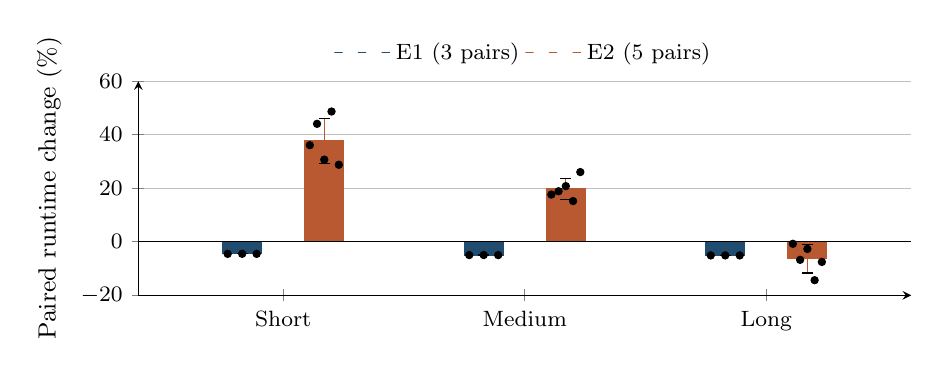
\begin{tikzpicture}\begin{axis}[width=.94\linewidth,height=\plotheight,axis lines=left,tick label style={font=\footnotesize},label style={font=\small},legend style={font=\footnotesize,draw=none},xmin=-.6,xmax=2.6,ymin=-20,ymax=60,xtick={0,1,2},xticklabels={Short,Medium,Long},ylabel={Paired runtime change (\%)},legend style={at={(.5,1.03)},anchor=south,legend columns=2},ymajorgrids=true]
\addplot[ybar,bar width=\barwidth,fill=navy,draw=navy,error bars/.cd,y dir=both,y explicit] coordinates {(-0.17,-4.518702515943322) +- (0,0.013983612419588681) (0.83,-4.972759574002627) +- (0,0.01531263015113631) (1.83,-5.1080291189045575) +- (0,0.0006388687927925786)};\addlegendentry{E1 (3 pairs)}
\addplot[only marks,black,mark size=\pointsize,forget plot] coordinates {(-0.23,-4.530613890120525) (-0.17,-4.503305918400253) (-0.11000000000000001,-4.522187739309188) (0.77,-4.966771331058025) (0.83,-4.961345976988894) (0.8899999999999999,-4.990161413960962) (1.77,-5.107775364024343) (1.83,-5.107556113289411) (1.8900000000000001,-5.108755879399918)};
\addplot[ybar,bar width=\barwidth,fill=burnt,draw=burnt,error bars/.cd,y dir=both,y explicit] coordinates {(0.17,37.66690998422855) +- (0,8.54813252860203) (1.17,19.713397108644475) +- (0,4.078864128468423) (2.17,-6.42312058356128) +- (0,5.256522242165112)};\addlegendentry{E2 (5 pairs)}
\addplot[only marks,black,mark size=\pointsize,forget plot] coordinates {(0.11000000000000001,36.10902959910078) (0.14,44.07596239300247) (0.17,30.693839452395775) (0.2,48.675331167208185) (0.23,28.780387309435525) (1.1099999999999999,17.63669140825637) (1.14,18.886500387722457) (1.17,20.795064347728964) (1.2,15.205769972306939) (1.23,26.042959427207634) (2.11,-0.7610558601580898) (2.14,-6.752098565253035) (2.17,-2.690881749745551) (2.1999999999999997,-14.371718841826734) (2.23,-7.539847900822994)};
\addplot[black,no marks,forget plot] coordinates {(-.6,0) (2.6,0)};
\end{axis}\end{tikzpicture}\end{column}
\begin{column}{.32\textwidth}\small
\textbf{Welch ANOVA $p$}\\Short: 0.000383\\Medium: 0.000173\\Long: 0.6057
\medskip
Compare paired percentage changes, with 3 versus 5 observations.
\medskip
Bars: mean. Whiskers: SD. Dots: pairs.
\medskip
\end{column}\end{columns}
\source{Updated Environment ANOVA, v8 rows. Lower runtime change favors Overloaded.}
\note{A low p value means the observed group means are difficult to reconcile with equality under the test assumptions. It is not a direct measure of the amount of environment variation or proof of environment causation.}
\end{frame}


\begin{frame}{Lower page-fault counts do not guarantee faster runtime}
\small\centering\begin{tabular}{lrlrl}\toprule
Run length & Peak memory & ANOVA $p$ & Minor faults & ANOVA $p$\\\midrule
Short & +4.39\% & $2.35\times10^{-9}$ & -77.52\% & $1.53\times10^{-4}$\\
Medium & +3.49\% & $4.21\times10^{-10}$ & -77.46\% & $5.74\times10^{-5}$\\
Long & +1.48\% & $5.24\times10^{-8}$ & -76.84\% & $8.59\times10^{-6}$\\
\bottomrule\end{tabular}\par
\medskip\raggedright\normalsize
\begin{itemize}\item E2 uses more peak memory and incurs fewer minor faults at every size.\item Short and medium runtime still worsens. These metrics do not identify a causal contribution to runtime.\item Major faults are zero for every E2 run. Their percentage change and ANOVA are undefined.\end{itemize}
\small Metric changes use $100(\bar O-\bar R)/\bar R$. These are selected diagnostic rows, including changes below the original 10\% display filter.
\source{Updated Metric ANOVA, v8 E2. n=5 per size; all p values unadjusted and exploratory.}
\end{frame}


\begin{frame}{Runtime outcomes across the shared analysis}
\centering\renewcommand{\plotheight}{4.1cm}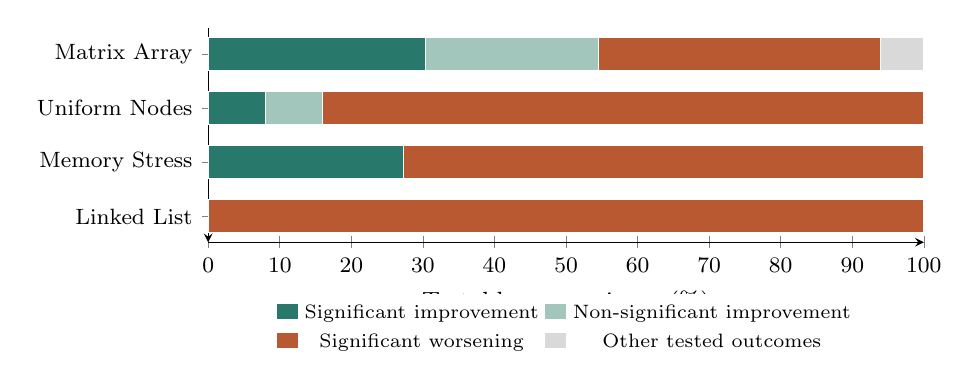
\begin{tikzpicture}\begin{axis}[width=.88\linewidth,height=\plotheight,axis lines=left,tick label style={font=\footnotesize},label style={font=\small},legend style={font=\footnotesize,draw=none},xbar stacked,bar width=12pt,xmin=0,xmax=100,y dir=reverse,ytick={0,1,2,3},yticklabels={Matrix Array,Uniform Nodes,Memory Stress,Linked List},xlabel={Testable comparisons (\%)},legend style={at={(.5,-.24)},anchor=north,legend columns=2,font=\scriptsize},enlarge y limits=.16]
\addplot[fill=teal,draw=white] coordinates {(30.303030303030305,0) (8.0,1) (27.272727272727273,2) (0.0,3)};\addlegendentry{Significant improvement}
\addplot[fill=lightteal,draw=white] coordinates {(24.242424242424242,0) (8.0,1) (0.0,2) (0.0,3)};\addlegendentry{Non-significant improvement}
\addplot[fill=burnt,draw=white] coordinates {(39.39393939393939,0) (84.0,1) (72.72727272727273,2) (100.0,3)};\addlegendentry{Significant worsening}
\addplot[fill=gray!30,draw=white] coordinates {(6.0606060606060606,0) (0.0,1) (0.0,2) (0.0,3)};\addlegendentry{Other tested outcomes}
\end{axis}\end{tikzpicture}
\par\scriptsize Testable comparisons: Matrix 33, Uniform Nodes 25, Memory Stress 11, Linked List 9. Each row has equal weight. Other tested outcomes include non-significant worsening and zero changes.
\source{Updated runtime chart. Uses all testable rows, not only the significant rows selected for tables.}
\end{frame}


\begin{frame}{Metric outcomes across the shared analysis}
\centering\renewcommand{\plotheight}{4.25cm}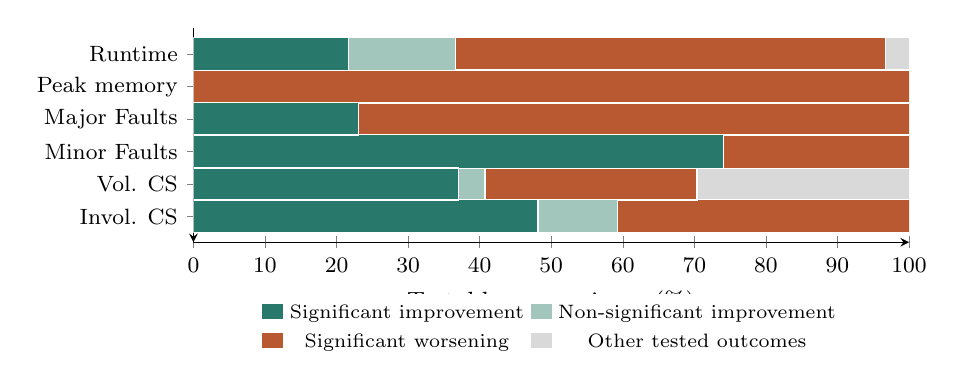
\begin{tikzpicture}\begin{axis}[width=.88\linewidth,height=\plotheight,axis lines=left,tick label style={font=\footnotesize},label style={font=\small},legend style={font=\footnotesize,draw=none},xbar stacked,bar width=12pt,xmin=0,xmax=100,y dir=reverse,ytick={0,1,2,3,4,5},yticklabels={Runtime,Peak memory,Major Faults,Minor Faults,Vol. CS,Invol. CS},xlabel={Testable comparisons (\%)},legend style={at={(.5,-.24)},anchor=north,legend columns=2,font=\scriptsize},enlarge y limits=.16]
\addplot[fill=teal,draw=white] coordinates {(21.666666666666668,0) (0.0,1) (23.076923076923077,2) (74.07407407407408,3) (37.03703703703704,4) (48.148148148148145,5)};\addlegendentry{Significant improvement}
\addplot[fill=lightteal,draw=white] coordinates {(15.0,0) (0.0,1) (0.0,2) (0.0,3) (3.7037037037037037,4) (11.11111111111111,5)};\addlegendentry{Non-significant improvement}
\addplot[fill=burnt,draw=white] coordinates {(60.0,0) (100.0,1) (76.92307692307692,2) (25.925925925925927,3) (29.62962962962963,4) (40.74074074074074,5)};\addlegendentry{Significant worsening}
\addplot[fill=gray!30,draw=white] coordinates {(3.3333333333333335,0) (0.0,1) (0.0,2) (0.0,3) (29.62962962962963,4) (0.0,5)};\addlegendentry{Other tested outcomes}
\end{axis}\end{tikzpicture}
\par\scriptsize CPU excluded. Denominators: Runtime 60, Peak memory 27, Major faults 13, Minor faults 27, Voluntary CS 27, Involuntary CS 27. Missing and untestable rows excluded.
\source{Updated metric chart. Aggregate outcomes mix campaigns and are descriptive, not a common-effect meta-analysis.}
\end{frame}


\begin{frame}{What the evidence cannot establish}
\begin{itemize}
\item Versions, machines, parameters, and compilers are not fully crossed. Workload changes can accompany environment changes.
\item Small samples limit precision and assumption checks. A non-significant Shapiro--Wilk or Levene test does not prove its assumption.
\item Fixed run order, background use, cache state, CPU frequency, and thermals can affect independence and fairness.
\item Runtime and resource totals do not separate arithmetic, allocator search, lock waiting, and memory-access costs.
\item Missing E1 raw resource observations and incomplete v8 list runs constrain further tests.
\end{itemize}
\source{Report Section XIV and updated v8 methods.}
\note{The main results use unadjusted v8 tests. The pthread report uses Tukey HSD for pairwise comparisons. The broad suite should be treated as exploratory rather than a single family of confirmatory hypotheses.}
\end{frame}


\begin{frame}{Conclusions supported by this study}
\begin{enumerate}
\item Representative workload patterns expose allocator tradeoffs without claiming exhaustive coverage.
\item V8 targets packed matrix rows, but its runtime benefit varies across the two measured groups.
\item Pthreads performance depends on implementation and environment. CMA can help the simpler implementation substantially.
\item Claims need effect sizes and inferential tests, with assumptions and sample sizes stated.
\item Code reading supports mechanisms. Dedicated profiling is still needed to attribute measured time to them.
\end{enumerate}
\source{Report and September 22 updates. Conclusions apply to tested configurations.}
\end{frame}

\begin{frame}{Team Member Contributions}
\begin{enumerate}
\item Jacob Nance
\item Mohamed Konsowa
\item Nicholas Johnson
\item Nicholas Hooper
\item Fernanda Gonzalez
\item Francisco Chagua
\end{enumerate}
\source{}
\end{frame}


\appendix

\begin{frame}{Appendix: paired ANOVA components for v8 E2}
\scriptsize\centering
\begin{tabular}{lrrrrrl}\toprule
Length & $SS_{
m cond}$ & $df_1$ & $SS_{
m error}$ & $df_2$ & $F$ & $p$\\\midrule
Short & 19,092.53 & 1 & 699.98 & 4 & 109.1038 & $4.75\times10^{-4}$\\
Medium & 107,601.20 & 1 & 3,475.31 & 4 & 123.8465 & $3.71\times10^{-4}$\\
Long & 124,347.03 & 1 & 70,491.33 & 4 & 7.0560 & 0.0566\\
\bottomrule\end{tabular}\par
\medskip\raggedright\normalsize
\[SS_{\rm cond}=\frac{n\bar d^2}{2},\qquad SS_{\rm error}=\frac{\sum_i(d_i-\bar d)^2}{2}\]
\[F=\frac{SS_{\rm cond}/1}{SS_{\rm error}/(n-1)}\]
\small This table shows the condition and error components used for the paired contrast. Subject variation is blocked out. The directional test is a separate analysis.
\source{Calculated from the five E2 pairs per size.}
\end{frame}


\begin{frame}{Appendix: reported pthread assumption and omnibus tests}
\small\centering
\begin{tabular}{lrrrr}\toprule
Environment & Shapiro--Wilk $p$ & Levene $p$ & ANOVA $F$ & ANOVA $p$\\\midrule
WSL & 0.0668 & 0.3466 & 1249.0073 & $3.560\times10^{-19}$\\
Linux & 0.5985 & 0.2418 & 4023.3356 & $3.148\times10^{-23}$\\
\bottomrule\end{tabular}\par
\medskip\raggedright\normalsize The omnibus tests report differences among the four method means. Tukey HSD identifies the pairs that differ.
\medskip
\small These values are copied from the report. Raw pthread observations were not supplied for independent recomputation. The report does not fully specify the grouping used for each normality diagnostic.
\source{Report Tables XIII, XVII, XIV and XVIII.}
\end{frame}


\begin{frame}{Appendix: evidence and reproducibility}
\small
\begin{itemize}
\item \textbf{Report:} \emph{Custom Memory Allocator Profiling}, supplied PDF, 31 pages. Code descriptions: III/VI. Pthreads: XII. Threats: XIV.
\item \textbf{Updated analysis:} supplied Tables workbook plus September 22 matrix CSV. E1 raw runtime values come from the prior v8 workbook.
\item \textbf{New v8 statistics:} paired ANOVA, exact sign tests, and exploratory Welch comparisons. E2 has five presumed pairs per size.
\item \textbf{Source conflicts:} the report’s older v8 tables/conclusion describe E1 only; current slides include E2. Its older chi-square flags do not incorporate the exact-test correction.
\item \textbf{Parameter conflict:} the report lists v2 medium matrix size as 800 in Table V and 900 in the inventory. Neither value is used for new v8 E2, whose CSV specifies 400.
\end{itemize}
\source{Method references: NIST Sign Test; SciPy ttest\_rel and f\_oneway documentation. Full source mapping in README.md.}
\end{frame}

\end{document}
